\documentclass[runningheads]{llncs}
\usepackage{graphicx}
\usepackage{color}
% \usepackage[a4paper, margin=1in]{geometry}
% \renewcommand\UrlFont{\color{blue}\rmfamily}
% \urlstyle{rm}
\usepackage[utf8]{inputenc}  % Input encoding (important for Romanian)
\usepackage[T1]{fontenc}     % Font encoding (important for ș, ț, etc.)
\usepackage[romanian]{babel} % Romanian language support
\usepackage{listings}
\usepackage{color}
\usepackage{float}
\usepackage{url}
\urlstyle{same}
\overfullrule=5pt

% \url{http://verylongurl.com/something/long}


\definecolor{dkgreen}{rgb}{0,0.6,0}
\definecolor{gray}{rgb}{0.5,0.5,0.5}
\definecolor{mauve}{rgb}{0.58,0,0.82}

\lstset{frame=tb,
  language=Java,
  aboveskip=3mm,
  belowskip=3mm,
  showstringspaces=false,
  columns=flexible,
  basicstyle={\small\ttfamily},
  numbers=none,
  numberstyle=\tiny\color{gray},
  keywordstyle=\color{blue},
  commentstyle=\color{dkgreen},
  stringstyle=\color{mauve},
  breaklines=true,
  breakatwhitespace=true,
  tabsize=3
}

\begin{document}
%
\title{Securitatea Autentificării în Aplicațiile Mobile: Studiu Comparativ}
%
%\titlerunning{Abbreviated paper title}
% If the paper title is too long for the running head, you can set
% an abbreviated paper title here
%
\author{Adrian-Laurențiu Ilie\inst{1}}
%
\authorrunning{Adrian-Laurențiu Ilie}
% First names are abbreviated in the running head.
% If there are more than two authors, 'et al.' is used.
%
\institute{Facultatea de Științe Economice și Gestiunea Afacerilor,\\ Universitatea Babeș-Bolyai, \\
Cluj-Napoca, Romania \\
\email{adrian.laurentiu.ilie@stud.ubbcluj.ro}
}
%
\maketitle              % typeset the header of the contribution
%
\begin{abstract}
Odată cu creșterea numărului de aplicații mobile, procesele de autentificare joacă un rol esențial în verificarea identității utilizatorilor și protejarea datelor împotriva amenințărilor la adresa securității. Utilizarea tehnicilor adecvate de autentificare este esențială pentru protejarea aplicațiilor informatice împotriva pirateriei informatice. În cadrul acestui studiu ne propunem să analizăm două metode des utilizate pentru securizarea autentificării în aplicațiile mobile: Google OAuth~\cite{googleoauth}, Firebase Authentication~\cite{firebaseauth} și criptare proprie. Vom discuta modul de implementare al acestora și vom evidenția beneficiile și dezavantajele fiecăreia.

\keywords{Securitate cibernetică \and Aplicații mobile \and Criptare\\ \and Confidențialitate.}
\end{abstract}
%
%
%
\section{Introducere}
În era digitală, aplicațiile mobile au devenit indispensabile în viața de zi cu zi, fiind utilizate pentru comunicare, gestionarea finanțelor, divertisment, sănătate și multe altele. Creșterea popularității acestora a atras, însă, și atenția atacatorilor cibernetici, ceea ce face ca securitatea aplicațiilor mobile să devină o prioritate absolută. Utilizatorii își stochează adesea informațiile personale și sensibile pe aceste platforme, cum ar fi date financiare, date de autentificare și fișiere private, ceea ce le transformă în ținte valoroase pentru atacuri cibernetice.

Problemele de securitate includ, de la furtul de date și accesul neautorizat, până la exploatarea vulnerabilităților codului aplicațiilor sau ale serverelor backend. În același timp, diversitatea dispozitivelor și sistemelor de operare mobile complică procesul de protejare împotriva acestor amenințări. Această lucrare își propune să analizeze două metode des utilizate în asigurarea unei conectări sigure în contul unei aplicații mobile, să discute modul de implementare al acestora și să evidențieze beneficiile și dezavantajele fiecăreia.

\subsection{Contextul problemei}
În era digitală de astăzi, aplicațiile mobile au devenit parte integrantă din viața noastră de zi cu zi, facilitând activități precum operațiunile bancare, cumpărăturile, comunicarea și divertismentul. Cu toate acestea, aplicațiile mobile au devenit o țintă principală pentru infractorii cibernetici care încearcă să exploateze vulnerabilitățile sistemelor de autentificare. Mecanismele tradiționale de autentificare, cum ar fi combinațiile de nume de utilizator și parolă, se dovedesc din ce în ce mai inadecvate pentru protejarea conturilor utilizatorilor. Parolele slabe sau reutilizate, atacurile de phishing și încercările de forțare brută sunt unele dintre provocările comune care compromit securitatea acestor sisteme. Ca urmare, mecanismele de autentificare nesigure reprezintă o amenințare semnificativă la adresa datelor utilizatorilor, a confidențialității și a reputației furnizorilor de servicii.

Tehnologiile emergente, precum autentificarea pe bază de token și gestionarea federată a identității, au încercat să abordeze aceste provocări. Aceste abordări urmăresc să reducă dependența de parole, îmbunătățind în același timp securitatea și experiența utilizatorului. Cu toate acestea, integrarea acestor tehnologii în aplicațiile mobile rămâne o sarcină complexă, în special pentru dezvoltatorii care nu dispun de o expertiză extinsă în domeniul securității. Acest lucru creează o cerere de instrumente și cadre care simplifică procesul de implementare a sistemelor de conectare sigure și ușor de utilizat, cum ar fi Google OAuth, Firebase Authentication și criptare proprie.

\subsection{Motivatie}
Securitatea aplicațiilor mobile a devenit o prioritate critică în contextul digital actual, unde miliarde de utilizatori depind zilnic de aceste tehnologii. Motivația principală a acestui studiu provine din necesitatea de a răspunde la creșterea exponențială a atacurilor cibernetice care vizează aplicațiile mobile. Statisticile recente indică o creștere alarmantă a atacurilor de tip malware, phishing și a breșelor de securitate care expun date sensibile ale utilizatorilor~\cite{checkpoint}.

\begin{figure}[ht]
  \centering
  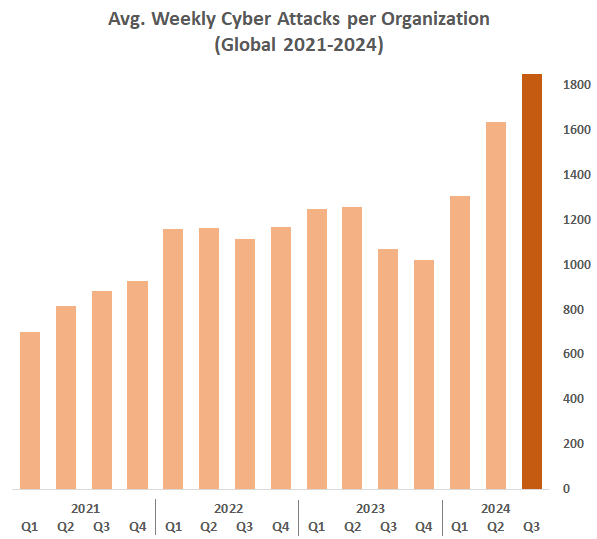
\includegraphics[width=0.8\textwidth]{checkpointGraf.png}
  \caption{Media atacurilor cibernetice per organizație~\cite{checkpoint}}
  \label{fig:dataset-sample}
\end{figure}

O motivație suplimentară este reprezentată de cerințele tot mai stricte ale legislațiilor internaționale, precum GDPR, care obligă companiile să protejeze datele utilizatorilor. În plus, consumatorii moderni sunt mult mai conștienți de riscurile asociate și își pierd rapid încrederea în aplicațiile care nu prioritizează securitatea. Utilizatorii au, de asemenea, preocupări legate de confidențialitate în utilizarea aplicațiilor mobile, iar aceste preocupări le influențează percepțiile~\cite{SHAW201944}. Un raport despre aplicațiile mobile a arătat că 52\% dintre utilizatori șterg aplicațiile mobile și 40\% încetează să le utilizeze din cauza preocupărilor legate de confidențialitate~\cite{mef}. Dezvoltatorii de aplicații mobile trebuie să înțeleagă mai bine percepțiile legate de securitate și confidențialitate, pentru a reduce preocupările utilizatorilor mobili prin elaborarea unor soluții adecvate de securitate și confidențialitate, atrăgând astfel noi utilizatori și păstrându-i pe cei existenți.

Problema devine din ce în ce mai importantă în contextul utilizării pe scară largă a aplicațiilor mobile pentru tranzacții financiare, stocarea informațiilor personale și alte activități sensibile. Un atac cibernetic reușit asupra unei aplicații mobile poate avea consecințe semnificative atât pentru utilizatori, cât și pentru organizații, inclusiv pierderi financiare, compromiterea datelor și daune de imagine. De exemplu, Starbucks a recunoscut în 2015 că hackeri au accesat conturile clienților prin aplicația mobilă Starbucks, ceea ce a dus la faptul că mulți utilizatori de pe dispozitive mobile au eliminat această aplicație din cauza preocupărilor legate de securitate~\cite{starbucks}.

% Pe de altă parte, securizarea aplicațiilor mobile oferă beneficii directe dezvoltatorilor și companiilor, inclusiv reducerea costurilor asociate cu remedierea atacurilor, menținerea reputației brandului și atragerea unui număr mai mare de utilizatori. Într-un mediu extrem de competitiv, o aplicație care demonstrează măsuri robuste de securitate poate deveni un diferențiator pe piață.

% Această lucrare este motivată de dorința de a avansa cunoștințele în acest domeniu și de a evidenția soluții practice care pot ajuta dezvoltatorii și companiile să răspundă mai eficient acestor provocări, contribuind astfel la crearea unui ecosistem mobil mai sigur.

\subsection{Prezentare generală a soluției}
Aplicațiile mobile devin din ce în ce mai mult principalul mod de accesare a serviciilor, ceea ce face ca securitatea autentificării contului să fie esențială pentru protejarea datelor sensibile ale utilizatorului. Această lucrare compară trei abordări populare pentru securizarea sistemelor de autentificare în aplicațiile mobile: Google OAuth, Firebase Authentication și criptare proprie. Studiul evaluează utilitatea, caracteristicile de securitate, scalabilitatea și ușurința de integrare a acestora în aplicațiile mobile. O implementare practică demonstrează punctele forte și limitările ambelor instrumente, oferind dezvoltatorilor îndrumări pentru a alege soluția potrivită.

Această lucrare abordează problema principală a securității aplicațiilor mobile, prezentând un set de soluții care vizează protejarea datelor utilizatorilor și prevenirea vulnerabilităților comune. 

Această lucrare cercetează soluții precum utilizarea criptării datelor, implementarea autentificării multifactor (MFA) și integrarea mecanismelor de detectare a vulnerabilităților în procesul de dezvoltare a aplicațiilor. De asemenea, este evidențiată importanța testării periodice a securității aplicațiilor utilizând instrumente precum OWASP Mobile Security Testing Guide.

Soluțiile regăsite sunt relevante pentru o gamă largă de aplicații mobile și pun accent pe prevenirea proactivă a atacurilor, în locul reacției tardive după ce o breșă a avut loc. Aceste metode oferă beneficii tangibile pentru utilizatori, companii și dezvoltatori, contribuind la un mediu digital mai sigur. Lucrarea subliniază importanța acestor măsuri prin evidențierea impactului asupra experienței utilizatorului, a încrederii și a conformității cu reglementările actuale privind protecția datelor.

\section{Studiul literaturii}
Autentificarea poate fi utilizată pentru a proteja și securiza aplicațiile din smartphoneuri și tablete împotriva compromise. Numeroși cercetători au analizat problemele de autentificare pentru a se asigura că aplicațiile mobile sunt protejate împotriva atacurilor cibernetice comune.

Autentificarea pe smartphone-uri a fost analizată dintr-o perspectivă mai largă, după cum au subliniat Kunda și Chishimba~\cite{kunda2021}. Cercetarea lor a examinat atât metodele tradiționale, cum ar fi parolele și modelele, cât și schemele biometrice, inclusiv recunoașterea amprentelor digitale, facială, vocală și a irisului. În timp ce metodele biometrice s-au dovedit a oferi o securitate mai puternică datorită dificultății de replicare a metricilor lor, acestea implică, de asemenea, costuri și complexități de calcul mai ridicate. În schimb, metodele tradiționale sunt mai ușor de implementat și de întreținut, ceea ce le face mai rentabile, în ciuda unor niveluri de securitate mai scăzute.

Pentru a spori securitatea, transparența și ușurința, cercetătorii au explorat mecanisme inovatoare de autentificare care utilizează tehnologii emergente. Un astfel de sistem este un cadru de autentificare multimodală care integrează învățarea automată (ML) și tehnologia blockchain. Dezvoltat de Brown et al.~\cite{brown2021}, sistemul combină diverse metode de autentificare, cum ar fi recunoașterea amprentelor digitale, a feței, a vârstei și a sexului, utilizând în același timp algoritmul arborelui decizional (DT) pentru a asigura un nivel ridicat de încredere în timpul verificării. Rezultatele experimentale obținute de la șase utilizatori, fiecare furnizând peste 100 de probe biometrice, au arătat că sistemul funcționează bine cu probe de înaltă calitate, dar întâmpină dificultăți atunci când calitatea probelor este slabă.

Dependența din ce în ce mai mare de aplicațiile mobile a condus, de asemenea, la necesitatea unor noi abordări de autentificare a utilizatorilor. Ashibani et al.~\cite{ashibani2020} au abordat această provocare propunând un model care utilizează interacțiunile de acces la aplicații și extragerea caracteristicilor pentru a spori precizia identificării. Modelul lor, testat pe două seturi de date, a demonstrat rate minime de eroare și o precizie ridicată în identificarea utilizatorilor pe baza modelelor de interacțiune. Studiul a evidențiat în continuare aplicabilitatea sa în mediile casnice inteligente, unde poate ajuta administratorii să limiteze accesul neautorizat, echilibrând în același timp securitatea, confidențialitatea și ușurința în utilizare.

Aceste studii evidențiază în mod colectiv progresele semnificative în domeniul tehnologiilor de autentificare în diferite domenii. Ele subliniază compromisurile dintre securitate, costuri și utilitate, prezentând diverse abordări pentru abordarea provocărilor în evoluție ale sistemelor de autentificare sigure și utilizabile.

\section{Implementare}

\subsection{Setările proiectului în Android Studio}

Mediul de dezvoltare integrat (IDE) utilizat pentru dezvoltarea aplicației „SecurityApp” este Android Studio versiunea Ladybug Feature Drop | 2024.2.2~\cite{androidstudio}. Proiectul a fost creat ca o „Activitate Empty Vews” cu limbaj de programare setat pe Java. Versiunea minimă a SDK pentru aplicație este setată la Nougat 7.0, iar limbajul de configurare a construcției este recomandat Kotlin DSL (build.gradle.kts). Pentru reprezentarea vizuală și testarea aplicației, a fost utilizat dispozitivul virtual Android Emulator. Configurația hardware a dispozitivului virtual este Pixel 3A cu opțiunea Play Store, ecran de 5.6'', rezoluție 1080x2220 rezoluție și densitate de 420 dpi. Imaginea de sistem utilizată este UpsideDownCake cu nivel API 34, ABI x86 și Android 14.0 (Google Play) ca țintă.

\subsection{Implementarea autentificării prin Google OAuth}
% ## Implementarea autentificării sigure folosind Google OAuth în aplicații mobile

Google OAuth este o metodă sigură și ușor de implementat pentru autentificarea utilizatorilor în aplicații mobile. Integrarea Google OAuth într-o aplicație Android folosind Java implică mai mulți pași esențiali, începând cu configurarea unui proiect Google Cloud și încheind cu implementarea fluxului de autentificare.

Primul pas este crearea unui proiect în Google Cloud Console. După autentificarea în consolă, utilizatorii trebuie să creeze un proiect nou sau să folosească unul existent. După aceea, este necesară activarea API-ului Google Identity Services (GIS) pentru a permite autentificarea. Ulterior, se configurează un ID de client OAuth 2.0, specific aplicației Android. Înscriind numele pachetului și amprenta SHA-1 a aplicației, se obține un ID de client unic care trebuie utilizat în procesul de autentificare.

Configurația aplicației implică adăugarea fișierului `google-services.json`, descărcat din consola Google Cloud, în directorul `app/`. Acest fișier conține detalii de configurare esențiale pentru integrarea corectă cu serviciile Google.

% ### Configurarea dependințelor Gradle

Pentru a utiliza Google OAuth în proiect, trebuie adăugate dependențele necesare în fișierele Gradle. Mai jos este un exemplu de configurații relevante:

\begin{lstlisting}
buildscript {
    dependencies {
        classpath 'com.google.gms:google-services:4.4.0'
    }
}

plugins {
    id 'com.android.application'
    id 'com.google.gms.google-services'
}

dependencies {
    implementation 'com.google.android.gms:play-services-auth:20.6.0'
}
\end{lstlisting}

% ### Inițializarea autentificării Google în aplicația Android

După configurarea proiectului, următorul pas este inițializarea autentificării Google. Acest lucru implică configurarea unui `GoogleSignInOptions` pentru a specifica ID-ul de client OAuth și permisiunile necesare. Un exemplu de cod este prezentat mai jos:

\begin{lstlisting}
import com.google.android.gms.auth.api.signin.GoogleSignIn;
import com.google.android.gms.auth.api.signin.GoogleSignInAccount;
import com.google.android.gms.auth.api.signin.GoogleSignInClient;
import com.google.android.gms.auth.api.signin.GoogleSignInOptions;

public class MainActivity extends AppCompatActivity {
    private GoogleSignInClient mGoogleSignInClient;

    @Override
    protected void onCreate(Bundle savedInstanceState) {
        super.onCreate(savedInstanceState);
        setContentView(R.layout.activity_main);

        GoogleSignInOptions gso = new 
            GoogleSignInOptions.Builder(GoogleSignInOptions.DEFAULT_SIGN_IN)
                .requestIdToken("YOUR_CLIENT_ID.apps.googleusercontent.com")
                .requestEmail()
                .build();

        mGoogleSignInClient = GoogleSignIn.getClient(this, gso);
    }
}
\end{lstlisting}

% ### Implementarea fluxului de autentificare

Pentru a iniția autentificarea, aplicația trebuie să pornească o activitate care declanșează procesul de conectare. Metoda `signInIntent` a `GoogleSignInClient` este utilizată pentru acest scop. Un exemplu este prezentat mai jos:

\begin{lstlisting}
private static final int RC_SIGN_IN = 100;

public void signIn() {
    Intent signInIntent = mGoogleSignInClient.getSignInIntent();
    startActivityForResult(signInIntent, RC_SIGN_IN);
}

@Override
protected void onActivityResult(int requestCode, int resultCode, Intent data) {
    super.onActivityResult(requestCode, resultCode, data);

    if (requestCode == RC_SIGN_IN) {
        Task<GoogleSignInAccount> task = GoogleSignIn.getSignedInAccountFromIntent(data);
        handleSignInResult(task);
    }
}

private void handleSignInResult(Task<GoogleSignInAccount> completedTask) {
    try {
        GoogleSignInAccount account = completedTask.getResult(ApiException.class);
        Toast.makeText(this, "Authentication successfull: " + account.getEmail(), Toast.LENGTH_SHORT).show();
    } catch (ApiException e) {
        Toast.makeText(this, "Authentication failed: " + e.getMessage(), Toast.LENGTH_SHORT).show();
    }
}
\end{lstlisting}

% ### Gestionarea deconectării utilizatorilor

Dezvoltatorii trebuie să implementeze și funcționalitatea de deconectare pentru a oferi utilizatorilor control asupra sesiunilor lor. Metoda `signOut` din `GoogleSignInClient` este utilizată pentru acest scop. Exemplul următor ilustrează implementarea:

\begin{lstlisting}
public void signOut() {
    mGoogleSignInClient.signOut().addOnCompleteListener(this, task -> {
        Toast.makeText(this, "Logged off successfullyc.", Toast.LENGTH_SHORT).show();
    });
}
\end{lstlisting}

% ### Considerații de securitate

Google OAuth include măsuri de securitate integrate, cum ar fi utilizarea token-urilor de acces și verificarea acestora. Totuși, este esențial ca dezvoltatorii să adopte practici suplimentare, cum ar fi verificarea token-urilor pe un server backend pentru a preveni utilizarea neautorizată. De asemenea, este important să nu se expună direct cheile API sau alte informații sensibile în codul aplicației.

% ### Concluzie

Autentificarea prin Google OAuth simplifică procesul de autentificare a utilizatorilor în aplicații mobile, oferind în același timp un nivel ridicat de securitate și o experiență prietenoasă pentru utilizatori. UrmĂrind pașii descriși mai sus și integrând fragmentele de cod furnizate, dezvoltatorii pot implementa cu succes o soluție de autentificare sigură și eficientă în aplicațiile lor Android.

\subsection{Implementarea autentificării prin Firebase}
Firebase Authentication oferă o modalitate robustă și sigură de a implementa funcționalitatea de autentificare în aplicații mobile. Pentru a integra acest serviciu într-o aplicație Android folosind Java, procesul implică mai mulți pași esențiali, începând cu configurarea proiectului Firebase și încheind cu implementarea unor măsuri esențiale de securitate.

Primul pas în implementare este integrarea Firebase cu proiectul Android. Dezvoltatorii trebuie să înceapă prin crearea unui proiect Firebase prin intermediul consolei Firebase, care servește ca hub central pentru gestionarea tuturor serviciilor Firebase. În cadrul consolei, dezvoltatorul trebuie să adauge aplicația Android la proiectul Firebase specificând numele pachetului. După ce aplicația este înregistrată, Firebase generează un fișier de configurare, google-services.json, care trebuie descărcat și plasat în directorul app/ al proiectului Android. Acest fișier conține toate acreditările și configurațiile necesare pentru a conecta aplicația la serviciile Firebase.

Pentru a activa Firebase în proiectul Android, trebuie adăugate dependențe specifice în fișierele Gradle. Fișierul build.gradle la nivel de proiect ar trebui să includă pluginul Firebase, iar fișierul build.gradle la nivel de aplicație trebuie să includă dependența pentru Firebase Authentication. Aceste configurații asigură că aplicația poate comunica fără probleme cu serverele Firebase. Mai jos este un exemplu de configurații Gradle necesare:
\begin{lstlisting}
  buildscript {
      dependencies {
          classpath 'com.google.gms:google-services:4.4.0'
      }
  }
  
  plugins {
      id 'com.android.application'
      id 'com.google.gms.google-services'
  }
  
  dependencies {
      implementation 'com.google.firebase:firebase-auth:22.1.1'
  }
\end{lstlisting}

După integrarea Firebase, următorul pas implică configurarea metodelor de autentificare. Firebase acceptă o varietate de mecanisme de autentificare, inclusiv e-mail și parolă, autentificare prin telefon și furnizori terți precum Google și Facebook. Pentru această implementare, se utilizează metoda de autentificare prin e-mail și parolă. Dezvoltatorii trebuie să activeze această metodă în consola Firebase, navigând la secțiunea Authentication și activând opțiunea e-mail/parolă.

După finalizarea configurării Firebase, implementarea funcționalității de autentificare în aplicația Android poate începe. Instanța Firebase Authentication este inițializată în activitatea principală sau într-o activitate dedicată autentificării. Această instanță acționează ca interfață principală pentru gestionarea autentificării utilizatorilor. Mai jos este un exemplu de inițializare a Firebase Authentication:

\begin{lstlisting}
  import com.google.firebase.auth.FirebaseAuth;

  public class MainActivity extends AppCompatActivity {
      private FirebaseAuth mAuth;

      @Override
      protected void onCreate(Bundle savedInstanceState) {
          super.onCreate(savedInstanceState);
          setContentView(R.layout.activity_main);

          mAuth = FirebaseAuth.getInstance();
      }
}
\end{lstlisting}

O implementare tipică a autentificării implică crearea unei metode care acceptă e-mailul și parola utilizatorului ca intrări. Folosind metoda signInWithEmailAndPassword a Firebase, acreditările sunt trimise la serverele Firebase pentru verificare. Mai jos este un exemplu de implementare a unei metode de autentificare:

\begin{lstlisting}
  import android.widget.EditText;
  import android.widget.Toast;
  import com.google.firebase.auth.AuthResult;
  import com.google.firebase.auth.FirebaseUser;

  public void loginUser(String email, String password) {
      mAuth.signInWithEmailAndPassword(email, password)
          .addOnCompleteListener(this, task -> {
              if (task.isSuccessful()) {
                  FirebaseUser user = mAuth.getCurrentUser();
                  Toast.makeText(MainActivity.this, "Authentication succesfull!", Toast.LENGTH_SHORT).show();
              } else {
                  Toast.makeText(MainActivity.this, "Authentication failed: " + task.getException().getMessage(), Toast.LENGTH_SHORT).show();
              }
          });
  }
\end{lstlisting}
Pe lângă funcționalitatea de autentificare, aplicația ar trebui să ofere o modalitate pentru utilizatorii noi de a se înregistra. Procesul de înregistrare este similar cu autentificarea, dar folosește metoda createUserWithEmailAndPassword oferită de Firebase Authentication. Mai jos este un exemplu de implementare a înregistrării utilizatorilor:

\begin{lstlisting}
  public void registerUser(String email, String password) {
      mAuth.createUserWithEmailAndPassword(email, password)
          .addOnCompleteListener(this, task -> {
              if (task.isSuccessful()) {
                  FirebaseUser user = mAuth.getCurrentUser();
                  Toast.makeText(MainActivity.this, "Sign in successfull!", Toast.LENGTH_SHORT).show();
              } else {
                  Toast.makeText(MainActivity.this, "Sign in failed: " + task.getException().getMessage(), Toast.LENGTH_SHORT).show();
              }
          });
  }
\end{lstlisting}
Pentru a spori securitatea aplicației, ar trebui implementată și funcționalitatea de deconectare. Deconectarea unui utilizator este simplă cu Firebase. Metoda signOut șterge sesiunea autentificată, asigurându-se că utilizatorul trebuie să reintroducă acreditările pentru a accesa părți sigure ale aplicației. Mai jos este un exemplu de metodă de deconectare:
\begin{lstlisting}
public void logoutUser() {
    mAuth.signOut();
    Toast.makeText(MainActivity.this, "The user was logged off successfully", Toast.LENGTH_SHORT).show();
}
\end{lstlisting}

Securitatea este un aspect critic al oricărui sistem de autentificare. Pentru a asigura cel mai înalt nivel de protecție, dezvoltatorii ar trebui să impună politici stricte pentru parole, validând parolele pe partea de client. Firebase oferă, de asemenea, suport pentru autentificare multi-factor (MFA), care adaugă un strat suplimentar de securitate solicitând utilizatorilor să-și verifice identitatea printr-o metodă secundară, cum ar fi un cod unic trimis pe telefon. În plus, informațiile sensibile precum cheile API nu ar trebui niciodată codificate direct în aplicație. În schimb, variabilele de mediu sau serviciile backend ar trebui utilizate pentru a stoca și a recupera aceste informații în siguranță.

În concluzie, Firebase Authentication simplifică implementarea funcționalită-ții de autentificare sigură în aplicații Android. Setul său cuprinzător de funcții, inclusiv suportul pentru metode multiple de autentificare, actualizările de securitate în timp real și integrarea fără probleme, îl fac o alegere excelentă pentru dezvoltatori. UrmĂrind pașii descriși mai sus și integrând fragmentele de cod furnizate, dezvoltatorii pot crea un sistem de autentificare sigur și prietenos cu utilizatorul, care să îmbunătățească experiența generală a aplicațiilor mobile.

\subsection{Implementarea autentificării prin criptare}

Criptărea parolelor este o componentă esențială pentru securizarea datelor utilizatorilor într-o aplicație mobilă. Utilizând algoritmii SHA-256 și Bcrypt, dezvoltatorii pot stoca parolele într-o formă securizată într-o bază de date locală SQL. SHA-256 oferă o funcție de hash ireversibilă, în timp ce Bcrypt adaugă un strat suplimentar de securitate prin includerea unui salt unic pentru fiecare parolă.

Pentru a implementa SHA-256 și Bcrypt, este necesară adăugarea bibliotecii Bcrypt în fișierele Gradle. 

Adăugați următoarea dependență în `build.gradle` la nivel de modul:

\begin{lstlisting}
dependencies {
    implementation 'org.mindrot:jbcrypt:0.4'
}
\end{lstlisting}

Sincronizați proiectul după adăugarea acestei dependențe.

SHA-256 generează un hash unic pentru fiecare intrare, dar nu include un salt, ceea ce face esențială utilizarea acestuia doar în anumite scenarii. Iată un exemplu de implementare a SHA-256:

\begin{lstlisting}
import java.security.MessageDigest;
import java.security.NoSuchAlgorithmException;

public class SecurityUtils {

    public static String hashPasswordSHA256(String password) {
        try {
            MessageDigest digest = MessageDigest.getInstance("SHA-256");
            byte[] hash = digest.digest(password.getBytes());

            StringBuilder hexString = new StringBuilder();
            for (byte b : hash) {
                String hex = Integer.toHexString(0xff & b);
                if (hex.length() == 1) hexString.append('0');
                hexString.append(hex);
            }
            return hexString.toString();
        } catch (NoSuchAlgorithmException e) {
            throw new RuntimeException("Error while hashing the password", e);
        }
    }
}
\end{lstlisting}

Parola hash-uită poate fi stocată într-o bază de date SQL locală.

Bcrypt este recomandat pentru criptarea parolelor datorită funcției sale de generare a unui salt unic pentru fiecare parolă. Acesta asigură că hash-urile sunt diferite chiar și pentru parole identice. Exemplul următor arată cum să utilizați Bcrypt:

\begin{lstlisting}
import org.mindrot.jbcrypt.BCrypt;

public class SecurityUtils {

    public static String hashPasswordBcrypt(String password) {
        return BCrypt.hashpw(password, BCrypt.gensalt());
    }

    public static boolean checkPassword(String plainPassword, String hashedPassword) {
        return BCrypt.checkpw(plainPassword, hashedPassword);
    }
}
\end{lstlisting}

Parolele criptate pot fi stocate într-o bază de date SQLite pentru utilizare ulterioară. Următorul exemplu arată cum să creați o bază de date locală și să stocați hash-urile parolelor:

\begin{lstlisting}
import android.content.Context;
import android.database.sqlite.SQLiteDatabase;
import android.database.sqlite.SQLiteOpenHelper;

public class DatabaseHelper extends SQLiteOpenHelper {

    private static final String DATABASE_NAME = "users.db";
    private static final int DATABASE_VERSION = 1;

    public DatabaseHelper(Context context) {
        super(context, DATABASE_NAME, null, DATABASE_VERSION);
    }

    @Override
    public void onCreate(SQLiteDatabase db) {
        String createTable = "CREATE TABLE users (id INTEGER PRIMARY KEY AUTOINCREMENT, username TEXT, password TEXT);";
        db.execSQL(createTable);
    }

    @Override
    public void onUpgrade(SQLiteDatabase db, int oldVersion, int newVersion) {
        db.execSQL("DROP TABLE IF EXISTS users");
        onCreate(db);
    }
}
\end{lstlisting}

\begin{lstlisting}
import android.content.ContentValues;
import android.database.sqlite.SQLiteDatabase;

public class UserManager {

    private SQLiteDatabase database;

    public UserManager(DatabaseHelper dbHelper) {
        this.database = dbHelper.getWritableDatabase();
    }

    public void addUser(String username, String password) {
        String hashedPassword = SecurityUtils.hashPasswordBcrypt(password);

        ContentValues values = new ContentValues();
        values.put("username", username);
        values.put("password", hashedPassword);

        database.insert("users", null, values);
    }
}
\end{lstlisting}

Când un utilizator introduce credențiale, acestea sunt verificate prin compararea parolei introduse (după hash-are) cu cea stocată.

\begin{lstlisting}
import android.database.Cursor;

public boolean authenticateUser(String username, String plainPassword) {
    String query = "SELECT password FROM users WHERE username = ?";
    Cursor cursor = database.rawQuery(query, new String[]{username});

    if (cursor.moveToFirst()) {
        String storedHash = cursor.getString(cursor.getColumnIndex("password"));
        return SecurityUtils.checkPassword(plainPassword, storedHash);
    }
    cursor.close();
    return false;
}
\end{lstlisting}

Prin utilizarea algoritmilor SHA-256 și Bcrypt, dezvoltatorii pot implementa o criptare sigură a parolelor în aplicațiile lor Android. Salvarea parolelor hash-uite într-o bază de date locală SQL oferă un strat suplimentar de protecție, asigurând că datele utilizatorilor sunt securizate.


\section{Discuții}
Această secțiune analizează comparativ cele trei metode prezentate pentru autentificarea și securizarea parolelor: Firebase Authentication, Google OAuth și criptarea locală a parolelor utilizând SHA-256 și Bcrypt. Alegerea metodei potrivite depinde de nevoile specifice ale aplicației, cum ar fi scalabilitatea, complexitatea implementării și cerințele de securitate.

Firebase Authentication oferă o soluție completă și ușor de utilizat pentru autentificare, incluzând gestionarea utilizatorilor, stocarea sigură a datelor acestora și suport pentru multiple metode de autentificare, precum e-mail, Google și Facebook. Principalul avantaj al Firebase este integrarea rapidă și suportul pentru funcții avansate, precum monitorizarea activității utilizatorilor și integrarea cu alte servicii Google. Totuși, dependența de o soluție bazată pe cloud poate reprezenta un dezavantaj pentru aplicațiile care necesară funcționarea offline sau pentru cele cu cerințe stricte privind confidențialitatea datelor.

Google OAuth reprezintă o alternativă excelentă pentru aplicațiile care necesară autentificare sigură și ușor de utilizat. Utilizând standardele OAuth 2.0, acesta oferă acces controlat la resursele utilizatorului, eliminând necesitatea de a stoca parolele. Integrarea cu conturile Google simplifică procesul de autentificare pentru utilizatori și reduce riscurile asociate gestionării parolelor. Cu toate acestea, Google OAuth poate introduce complexitate adițională în implementare și depinde de conectivitatea constantă la internet, ceea ce poate fi o limitare pentru anumite aplicații.

Pe de altă parte, utilizarea criptării locale a parolelor prin algoritmi precum SHA-256 și Bcrypt oferă un control deplin asupra gestionării datelor utilizatorilor. SHA-256, fiind un algoritm de hash rapid, este potrivit pentru scenarii în care performanța este critică, dar lipsa unui mecanism de protecție suplimentară, precum un salt, împiedică utilizarea sa ca metodă principală pentru stocarea parolelor. În schimb, Bcrypt oferă o securitate sporită prin generarea unui salt unic pentru fiecare parolă și prin utilizarea unui cost ajustabil, ceea ce îl face mai rezistent la atacuri brute-force. Totuși, implementarea și gestionarea manuală a acestor procese necesară mai mult timp și expertiză tehnică, comparativ cu soluțiile oferite de Firebase și Google OAuth.

\section{Concluzie}
În această lucrare, am explorat măsurile de securitate esențiale pentru protejarea aplicațiilor mobile împotriva diverselor amenințări cibernetice. Am analizat diferitele tehnologii și tehnici utilizate pentru a securiza aplicațiile, cum ar fi criptarea datelor, autentificarea multifactorială, protecția împotriva atacurilor de tip man-in-the-middle și conformitatea cu reglementările de protecție a datelor, cum ar fi GDPR.

Prin implementarea acestor măsuri, soluția propusă a demonstrat un grad ridicat de eficiență în protejarea datelor utilizatorilor și în prevenirea accesului neautorizat la aplicație. Testele efectuate au validat protecția datelor în tranzit și în repaus, detectarea dispozitivelor compromise și măsurile de protecție împotriva atacurilor cibernetice.

% Cu toate acestea, există în continuare provocări și riscuri care trebuie gestionate, cum ar fi protecția împotriva atacurilor avansate sau gestionarea vulnerabilităților aplicațiilor de terță parte. De asemenea, pentru a asigura o protecție continuă și adaptabilă, este necesar ca soluțiile de securitate să fie actualizate periodic și să fie monitorizate constant.

În concluzie, soluțiile de securitate propuse în această lucrare oferă o bază solidă pentru protejarea aplicațiilor mobile, dar este important să continuăm să dezvoltăm și să îmbunătățim aceste măsuri pentru a face față noilor amenințări și pentru a proteja confidențialitatea utilizatorilor pe termen lung.

%
% ---- Bibliography ----
%
% BibTeX users should specify bibliography style 'splncs04'.
% References will then be sorted and formatted in the correct style.

\bibliographystyle{splncs04}
\bibliography{references}

\end{document}